\documentclass[11pt]{article}

\parindent 0in
\parskip 0.0in

\def\setmarsing{
\voffset-0.59in
\hoffset-0.5in
\textwidth6.5in
\textheight9in}

\setmarsing

\usepackage{natbib}
\usepackage{color}
\usepackage[pdftex]{graphicx}
\usepackage{epsfig}
\usepackage{wrapfig}
\usepackage{sidecap}
\usepackage{subfig}
\usepackage{fancyhdr}  %header
\usepackage{amsmath,amsthm,amsfonts,amssymb}
\usepackage[T1]{fontenc}

%\numberwithin{equation}{section} %equation numbered as something like (3.1)

%%%% YOU CAN PUT YOUR OWN DEFINITIONS HERE
\newcommand{\equa}[1]{(\ref{eq:#1})}
\newcommand{\laeq}[1]{\label{eq:#1}}
\newcommand{\figu}[1]{\ref{fig:#1}}
\newcommand{\lafi}[1]{\label{fig:#1}}
\newcommand{\fmo}{\tilde{U}}
\newcommand{\fve}{\tilde{u}}
\newcommand{\Dt}{\Delta t}

\newcommand{\R}{\mathbb{R}}
\newcommand{\Z}{\mathbb{Z}}
\newcommand{\si}[1]{\rm\scriptscriptstyle{#1}}

\newcommand\p{\ensuremath{\partial}}
\newcommand\pdt{\ensuremath{\frac{\p}{\p t}}}
%\newcommand{\bm}[1]{\O{\boldmath $#1$}}

\def\be{\begin{equation}}
\def\bea{\begin{eqnarray}}
\def\ee{\end{equation}}
\def\eea{\end{eqnarray}}
\def\Ddt{\frac{D}{Dt}\;}
\def\Ddts{\frac{D^2}{Dt^2}\;}
\def\ddt{\frac{d}{dt}\,}

\def\cT{{\cal T}}
\def\cA{{\cal A}}
\def\cAB{{\cal AB}}
\def\cAC{{\cal AC}}
\def\cB{{\cal B}}
\def\cBC{{\cal BC}}
\def\cC{{\cal C}}
\def\cP{{\cal P}}
\def\cb{{\cal b}}
\def\cS{{\cal S}}
\def\cW{{\cal W}}
\def\cD{{\cal D}}
\def\cO{{\cal O}}
\def\cV{{\cal V}}
\def\cvs{{\cal v}}
\def\cF{{\cal F}}
\def\cvs{{\cal s}}
\def\cE{{\cal E}}

\def\kt{\tilde{k}}
\def\Ut{\tilde{U}}
\def\rhob{\bar{\rho}}

\def\twothird{\frac{2}{3}}
\def\half{\frac{1}{2}}
\def\third{\frac{1}{3}}
\def\fourthird{\frac{4}{3}}
\def\fourth{\frac{1}{4}}

\def\<{\langle}
\def\>{\rangle}
%%%% END OF YOUR DEFINITIONS 


\fancyhead[RE,RO]{\it LA-UR-14-20669}
\renewcommand{\headrulewidth}{0pt}
\pagestyle{fancy}%


\begin{document}

\begin{center}
\Large
{\color{blue}\bf The Johns Hopkins Turbulence Databases ({\em JHTDB})}
\end{center}

\normalsize

\begin{center}
\bf HOMOGENEOUS BUOYANCY DRIVEN TURBULENCE DATA SET
\end{center}

\vskip 0.2in


\begin{center}
{\em Data provenance:} D. Livescu$^1$ \\
{\em Database Ingest and Web Services:} C. Canada$^1$, K. Kanov$^2$, 
R. Burns$^2$ \& IDIES staff\\
{\em Visualization:} J. Pulido$^{1,3}$\\
$^1$Los Alamos National Laboratory, Los Alamos, NM 87544\\
$^2$Johns Hopkins University, Baltimore, MD 21218\\
$^3$University of California, Davis, CA 95616\\
\end{center}

\vskip 0.2in

The data is from a direct numerical simulation (DNS) of homogeneous buoyancy 
driven turbulence on a $1024^3$ periodic grid. The equations solved are the 
miscible two-fluid incompressible Navier-Stokes equations, which are obtained 
from the fully compressible Navier-Stokes equations with two species with 
different molar masses in the limit $c \rightarrow \infty$ ($c$ is the speed of
sound) such that the individual densities of the two fluids remain constant 
\cite{LR07,LR08,Livescu13}:

\begin{eqnarray}
\label{eq.01}
\pdt \rho + (\rho u_j)_{,j} &=& 0
\\
\label{eq.02}
\pdt (\rho u_i) + (\rho u_i u_j)_{,j} &=& -p_{,i}+\tau_ {ij,j}+
\frac{1}{Fr^2}\rho g_i
\\
\label{eq.div}
u_{j,j}  &=&  - \frac{1}{Re_0 Sc} (ln \rho)_{,jj},
\end{eqnarray}

\noindent
where $\rho$ is the density of the mixture (defined according to
$\rho = (Y_1/\rho_1+Y_2/\rho_2)^{-1}$ with $Y_1+Y_2=1$ being the mixture 
fractions and $\rho_1$ and $\rho_2$ the fluids' individual densities 
\cite{LR07}), $u_i$ is the mixture's velocity vector field and $p$ the 
pressure. The viscous stress is Newtonian with

\begin{equation}
\tau_{ij}=\frac{\rho}{Re_0}
[u_{i,j}+u_{j,i}-\twothird u_{k,k}\delta_{ij}]
\end{equation}

\noindent
Note that Eqs. (\ref{eq.01})-(\ref{eq.02}) are the usual continuity and 
momentum transport equations for compressible flows. Equations
(\ref{eq.01})-(\ref{eq.div}) describe the mixing, at any density ratio, between
incompressible materials or compressible materials in low speed, low 
acceleration flows, when the fluids participating in the mixing maintain 
quasi-constant microscopic densities. If the densities of the two fluids are 
commensurate, then the mixture density is close to its average value and 
Eqns. (\ref{eq.01})-(\ref{eq.div}) lead to the Boussinesq approximation
(see Ref. \cite{LR07} for the derivation). An example of DNS of such flow in 
the Boussinesq limit can be found in Ref. \cite{BCC92}. Note that the 
divergence of velocity is not zero for the non-Boussinesq case, as the specific
volume changes during mixing. 

The nondimensional parameters are the computational Reynolds number, $Re_0$, 
Schmidt number, $Sc$, and Froude number, $Fr$. $g_i$ are the components of the 
unit vector in the direction of gravity, $\vec{g}=(1,0,0)$, and the kinematic 
viscosity, $\nu_0=\mu/\rho$, and mass diffusion coefficient, $\cal{D}$, are 
assumed constant, such that $Sc$ is uniform throughout the flow. The 
independent variables are the time $t$ and space variables, $x_i$. Equations 
(\ref{eq.01})-(\ref{eq.div}) have periodic boundary conditions and the 
homogeneity of the fluctuating quantities is ensured by imposing mean zero 
velocity and constant mean pressure gradient \cite{LR07}. These conditions are 
similar to those encountered in the interior of the Rayleigh-Taylor mixing 
layer during the turbulent stage \cite{LRGDCC09}. Eqns. 
\ref{eq.01}-\ref{eq.div} are solved using a pseudo-spectral approach, with the 
skew-symmetric form of the advection terms to minimize aliasing errors, and the
third order predictor-corrector Adams-Bashforth-Moulton scheme coupled with a 
pressure projection method for time advancement. 

The simulation was performed with the variable-density version of the petascale
CFDNS code \cite{cfdns}. The two fluids are initialized as random blobs,
consistent with the homogeneity assumption. The flow starts from rest, with 
only a small amount of dilatational velocity necessary to satisfy condition
\ref{eq.div}, and turbulence is generated as the two fluids start moving in 
opposite directions due to differential buoyancy forces. However, as the fluids
become molecularly mixed, the buoyancy forces decrease and at some point the 
turbulence starts decaying. The database covers both the buoyancy driven 
increase in turbulence intensity as well as the buoyancy mediated turbulence 
decay. All averages are calculated as volume averages. Below, fluctuations
about the Reynolds averages are denoted by primes, while fluctuations about 
Favre (density weighted) averages are denoted by double primes.

\vskip 0.2in

{\bf Simulation parameters}

Domain: $2\ \pi \times 2\ \pi \times 2\ \pi$ (i.e. range of $x_1$, $x_2$, and
$x_3$ is $[0,2\pi ]$)

Grid: $1024^3$

Computational Reynolds number: $12,500$ (inverse of the non-dimensional 
kinematic viscosity, $1/\nu$)

Schmidt number: 1.0

Froude number: 1.0

Density of pure light fluid: $1.0$ (non-dimensional)

Density of pure heavy fluid: $1.0/0.95 \approx 1.105$ (non-dimensional)

Atwood number: 0.05

Mean density: $\approx 1.053$ (non-dimensional)

Initial density integral lengthscale: $\approx 1.382$ (non-dimensional)

Initial density variance: $\approx 0.002681$ (non-dimensional) 

Minimum DNS time step: $8 \times 10^{-4}$ (non-dimensional)

Maximum DNS time step: $2 \times 10^{-3}$ (non-dimensional)

Database time step: $4 \times 10^{-2}$ (non-dimensional)

Time stored: from $t=0$ to $t=40.56$ (1015 datafiles)


\vskip 0.2in

{\bf Flow statistics}

Maximum turbulent Reynolds number: 
$Re_t = \frac{\tilde{k}^2}{\nu \epsilon} \approx 17,765$

Time at maximum $Re_t$: $6.56$

Maximum Favre kinetic energy: $\tilde{k}= 
\frac{<\rho u_i'' u_i''>}{2 <\rho>} = 0.04186$ (at time $11.4$).

$\tilde{k}$ at maximum $Re_t$: $0.02388$

Maximum eddy turnover time: $\tau = \frac{\tilde{k}}{\epsilon}=77.63$
(at time $4.2$).

$\tau$ at maximum $Re_t$: $59.52$ and at maximum $\tilde{k}$: $12.82$.

Maximum turbulent kinetic energy dissipation: $\epsilon=0.005332$ (at time
$14.56$)

$\epsilon$ at maximum $Re_t$: $0.0004012$ and at maximum $\tilde{k}$: 
$0.003098$.

\vskip 0.2in

Several quantities from the simulation are shown in the figures below. Figures
1-5 show the time evolutions of turbulent Reynolds number, Favre turbulent 
kinetic energy, Reynolds stresses in the direction of gravity, 
$R_{vv}= <\rho u_1'' u_1''>$, and perpendicular to gravity, 
$R_{hh}= (<\rho u_2'' u_2''>+<\rho u_3'' u_3''>)/2$, and vertical mass 
flux, $a_v = <\rho u_1'>/<\rho>$, eddy turnover time, kinetic energy 
dissipation, density variance and density-specific volume correlation, 
respectively. Figure 6 shows shows the density PDF at different times. Finally,
figure 7 shows the 3-D power spectra of density, $E_{\rho\rho}$, vertical and 
horizontal velocities, $E_{vv}= E_{11}$ and $E_{hh}= (E_{22}+E_{33})/2$, and 
density vertical velocity co-spectrum, $E_{v\rho}$, at $t=6.56$ and $t=11.4$. 

\vskip 0.2in

{\bf Acknowledgments:} Los Alamos National Laboratory is operated by the Los 
Alamos National Security, LLC for the U.S. Department of Energy NNSA under 
contract no. DE-AC52-06NA25396. Computational resources for the simulation
described here were provided by LANL Institutional Computing (IC) Program.

%%%% BIBLIOGRAPHY
%\bibspacing=\dimen 100
\bibliographystyle{unsrt}
\bibliography{README-HBDT}

\vskip 0.2in

{\em * Note:}
The velocity divergence condition (Eq. \ref{eq.div}) in the simulation is 
enforced based on the spectral representation of the derivatives. The JHTDB 
analysis tools for gradients are based on finite differencing of various 
orders. Therefore, when evaluating the divergence using these spatially more 
localized derivative operators, a non-negligible error in the divergence is 
obtained, as expected.

\vskip 2in

\center

\begin{figure}[h]
\center{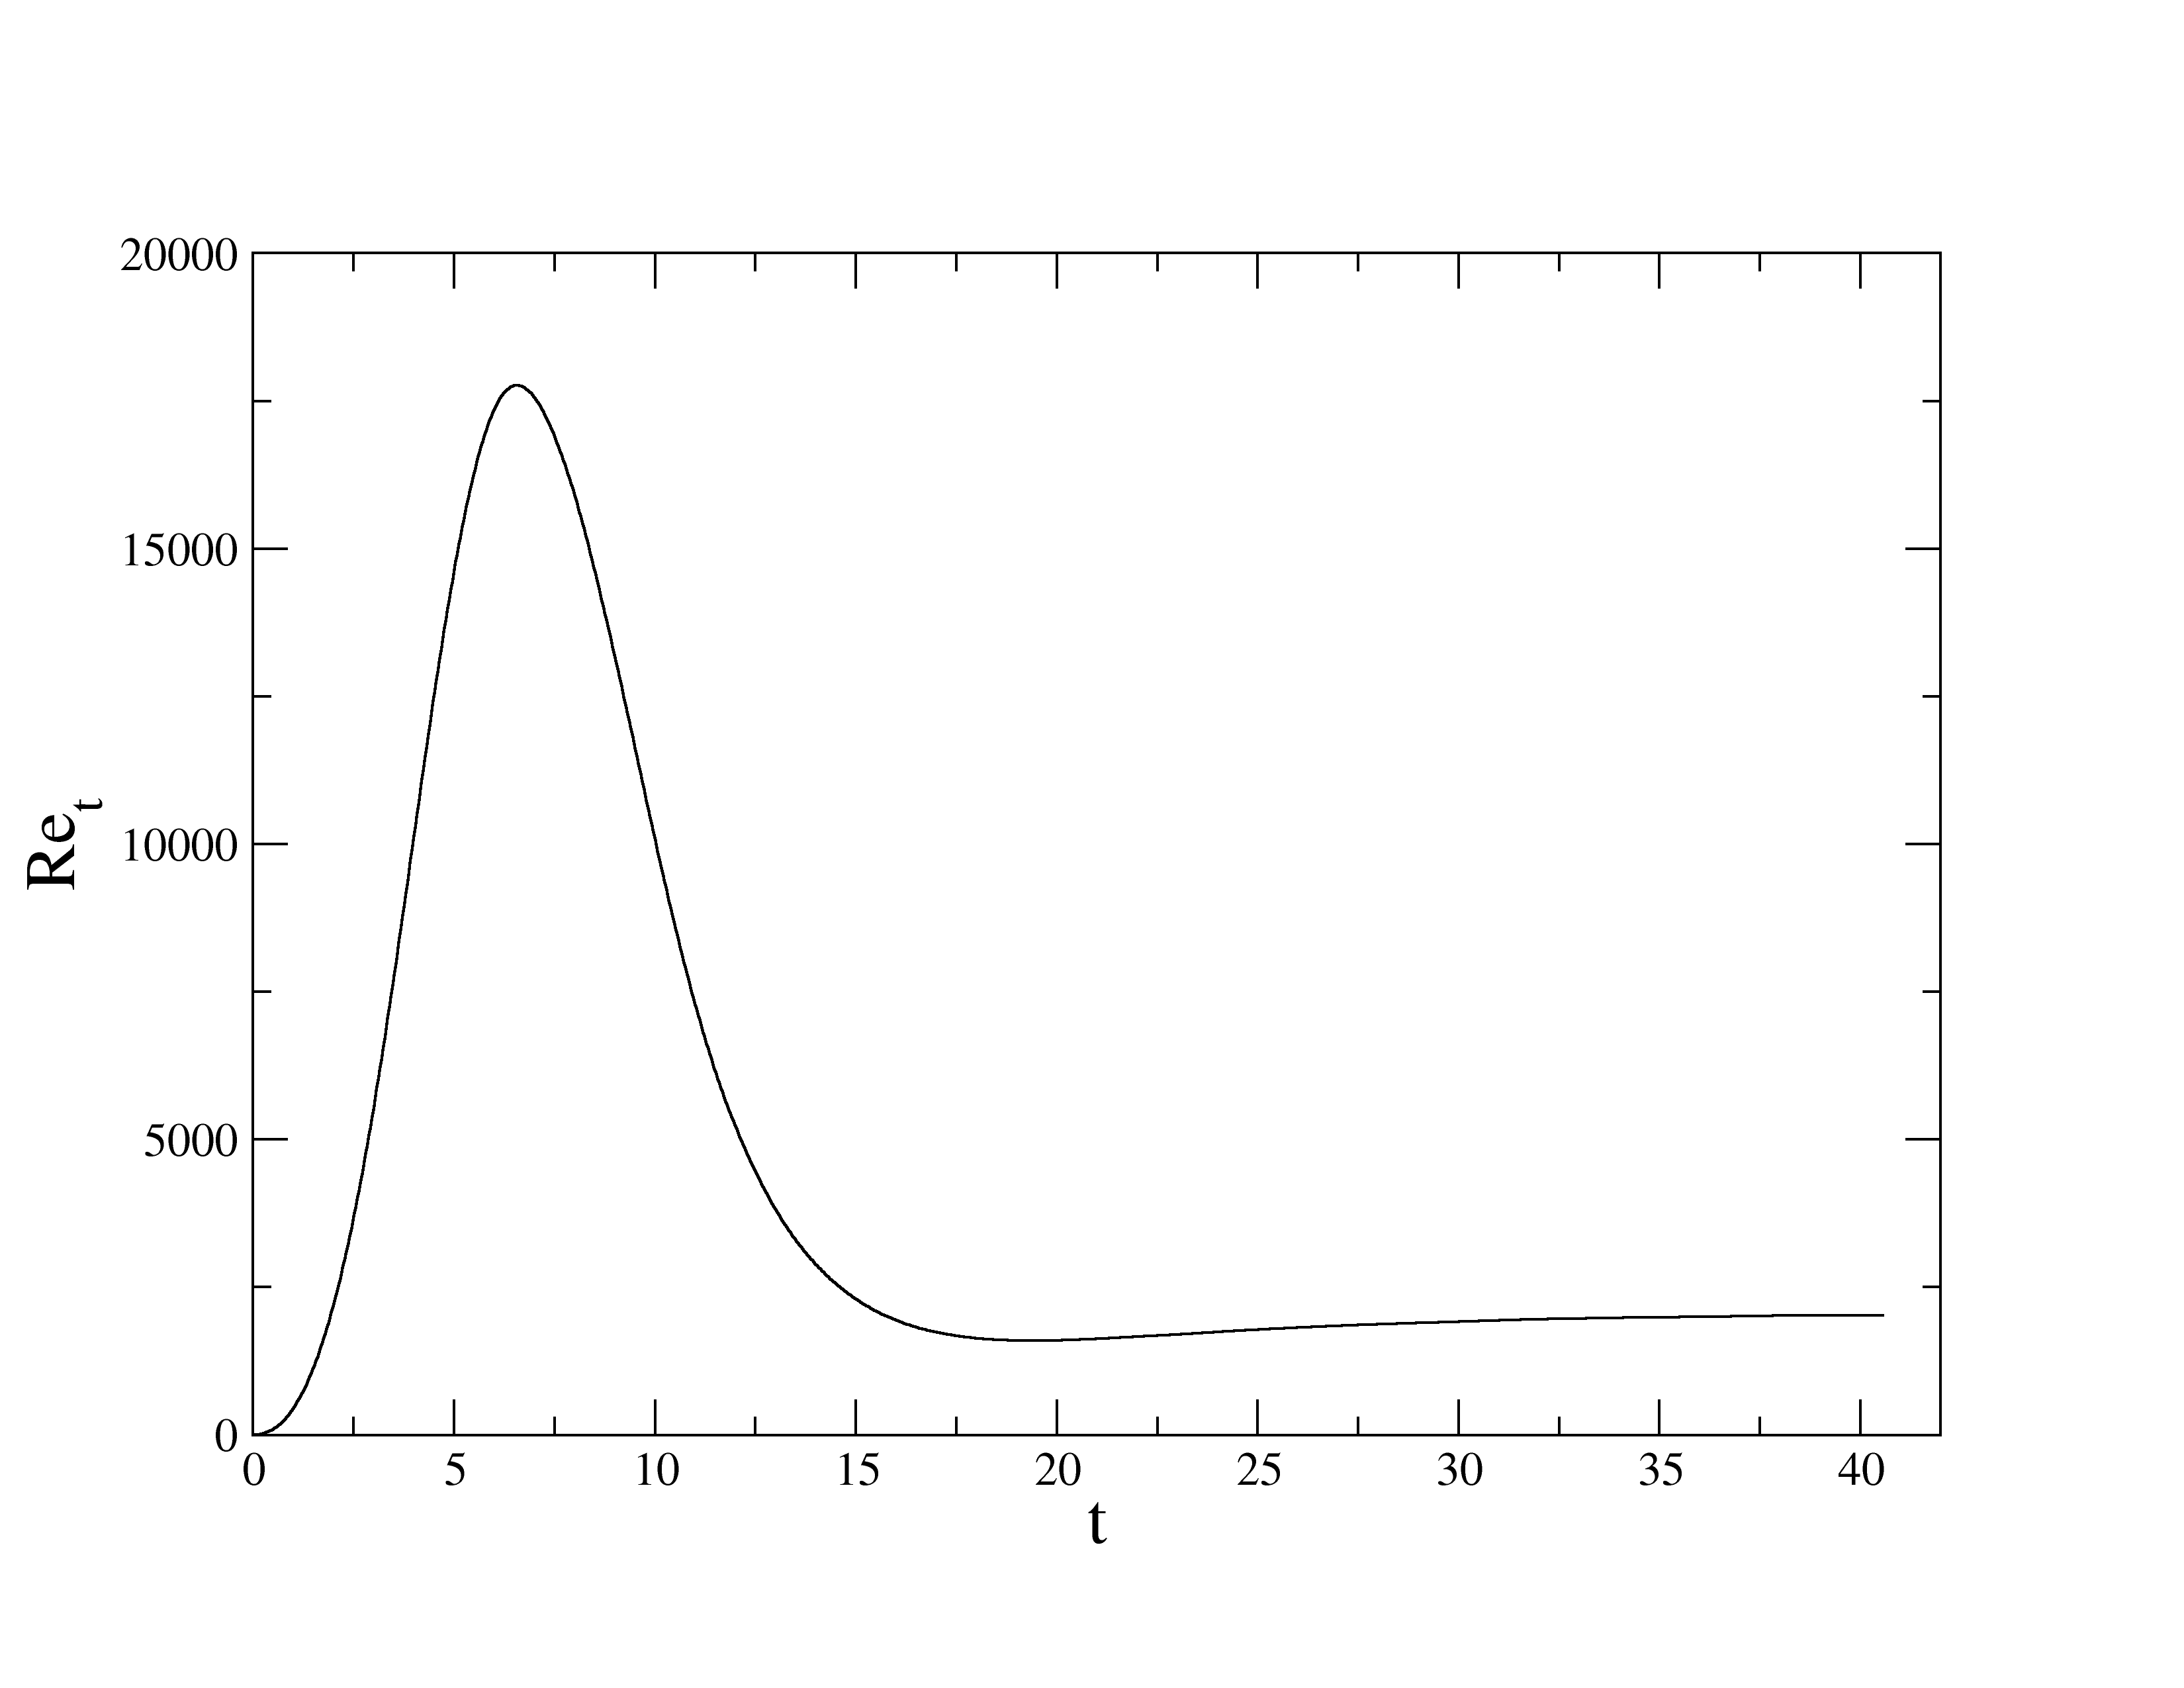
\includegraphics[width=4.5in,clip]{Ret.png}}
\caption{Evolution of turbulent Reynolds number.}
\label{figure1}
\end{figure}

\begin{figure}[h]
\center{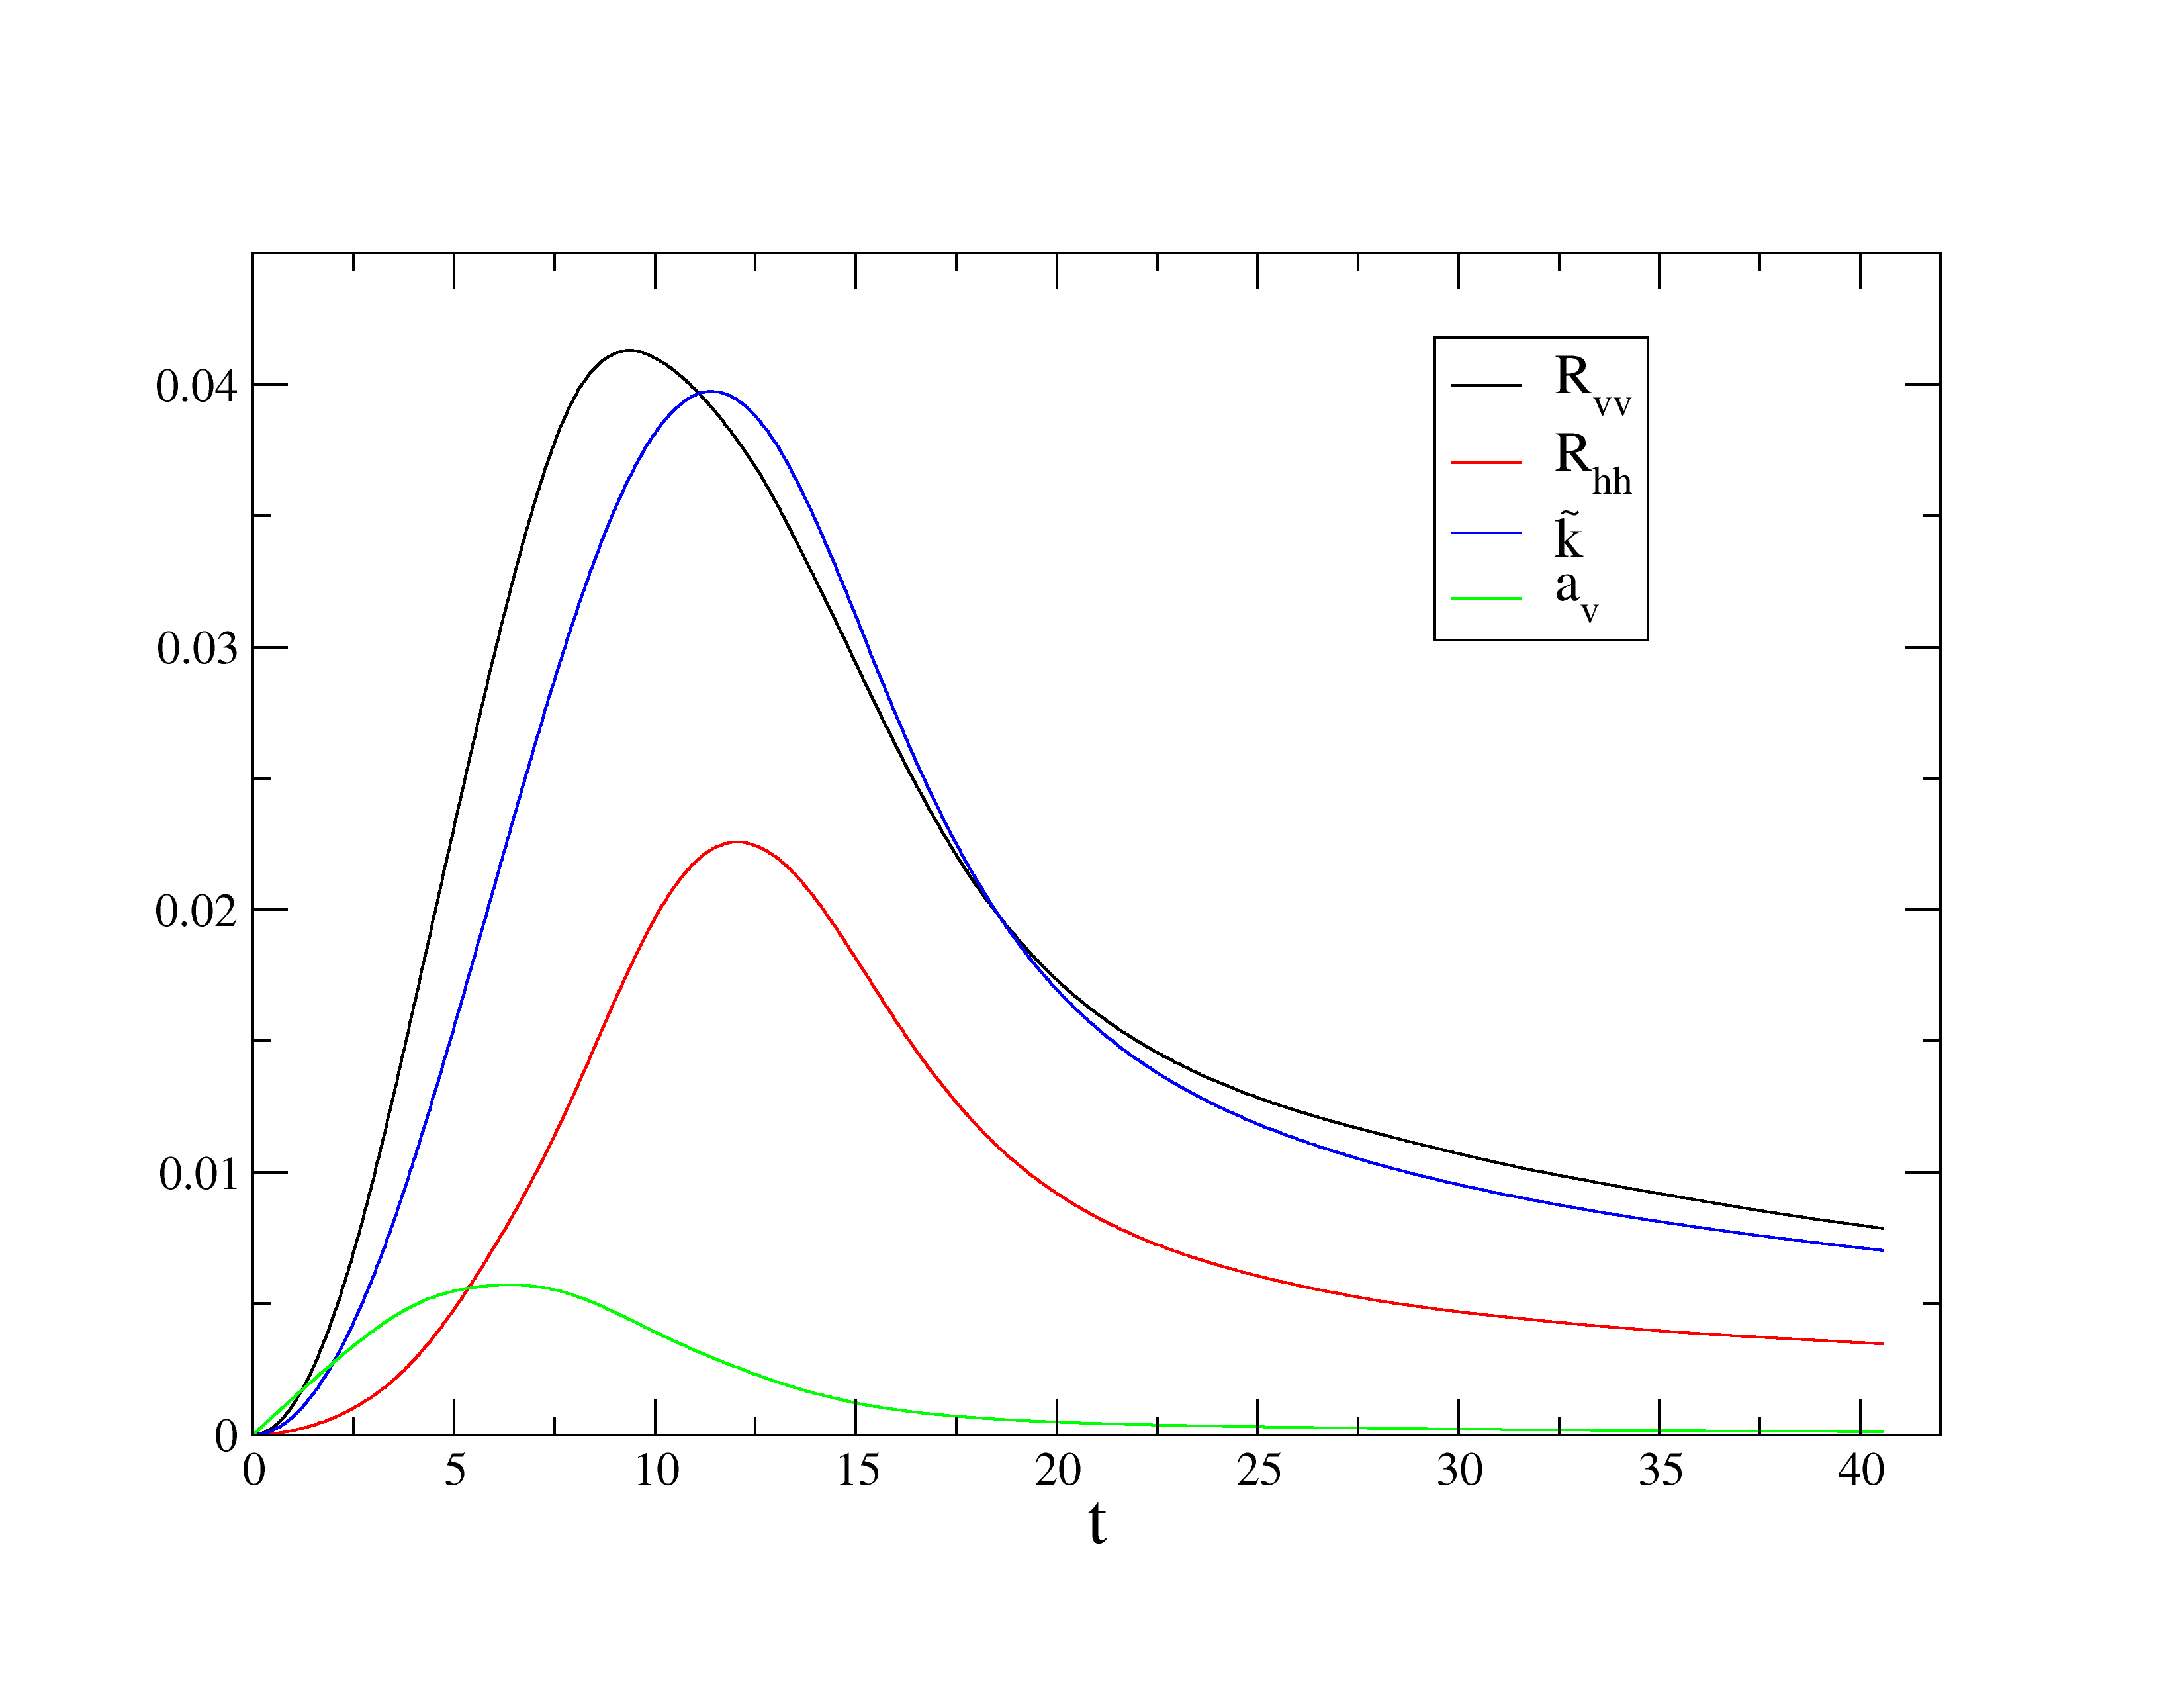
\includegraphics[width=4.5in,clip]{ktur.png}}
\caption{Evolution of Favre turbulent kinetic energy, vertical and horizontal 
Favre Reynolds stresses, $R_{vv}= <\rho u_1'' u_1''>$ and 
$R_{hh}= (<\rho u_2'' u_2''>+<\rho u_3'' u_3''>)/2$, and vertical mass 
flux, $a_v = <\rho u_1'>/<\rho>$.}
\label{figure2}
\end{figure}

\begin{figure}[h]
\center{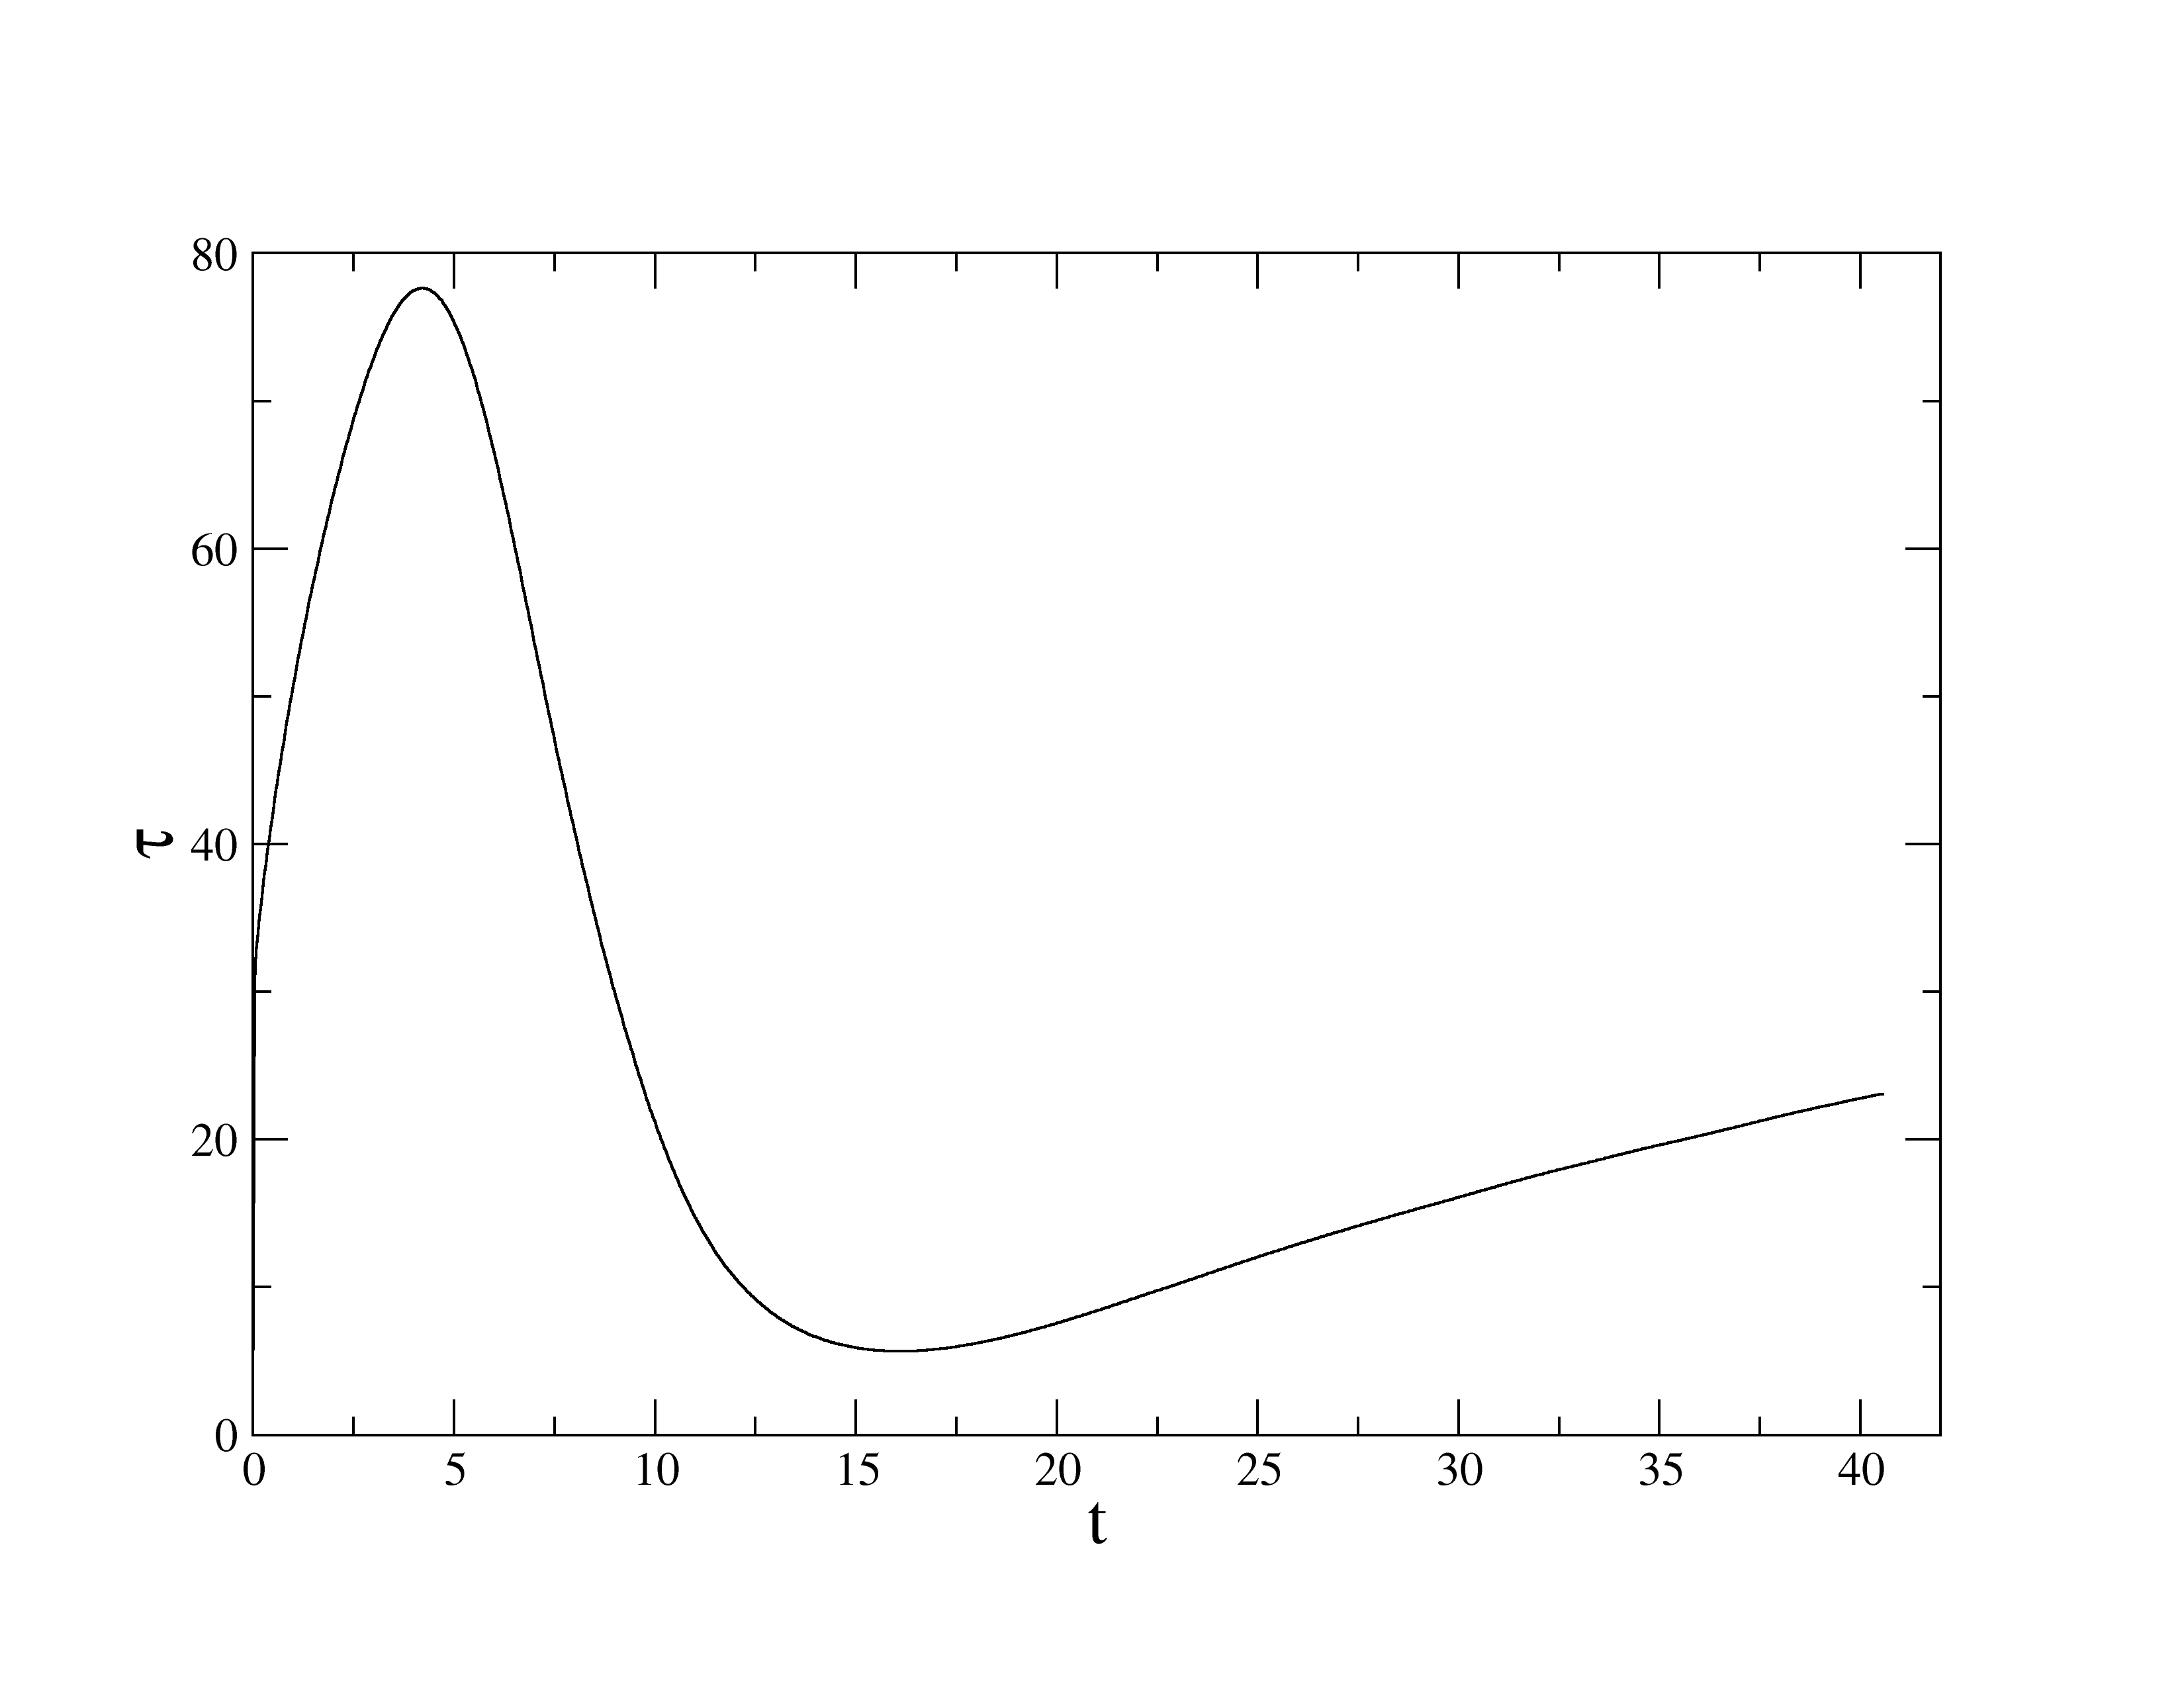
\includegraphics[width=4.5in,clip]{Taut.png}}
\caption{Evolution of eddy turnover time.}
\label{figure3}
\end{figure}

\begin{figure}[h]
\center{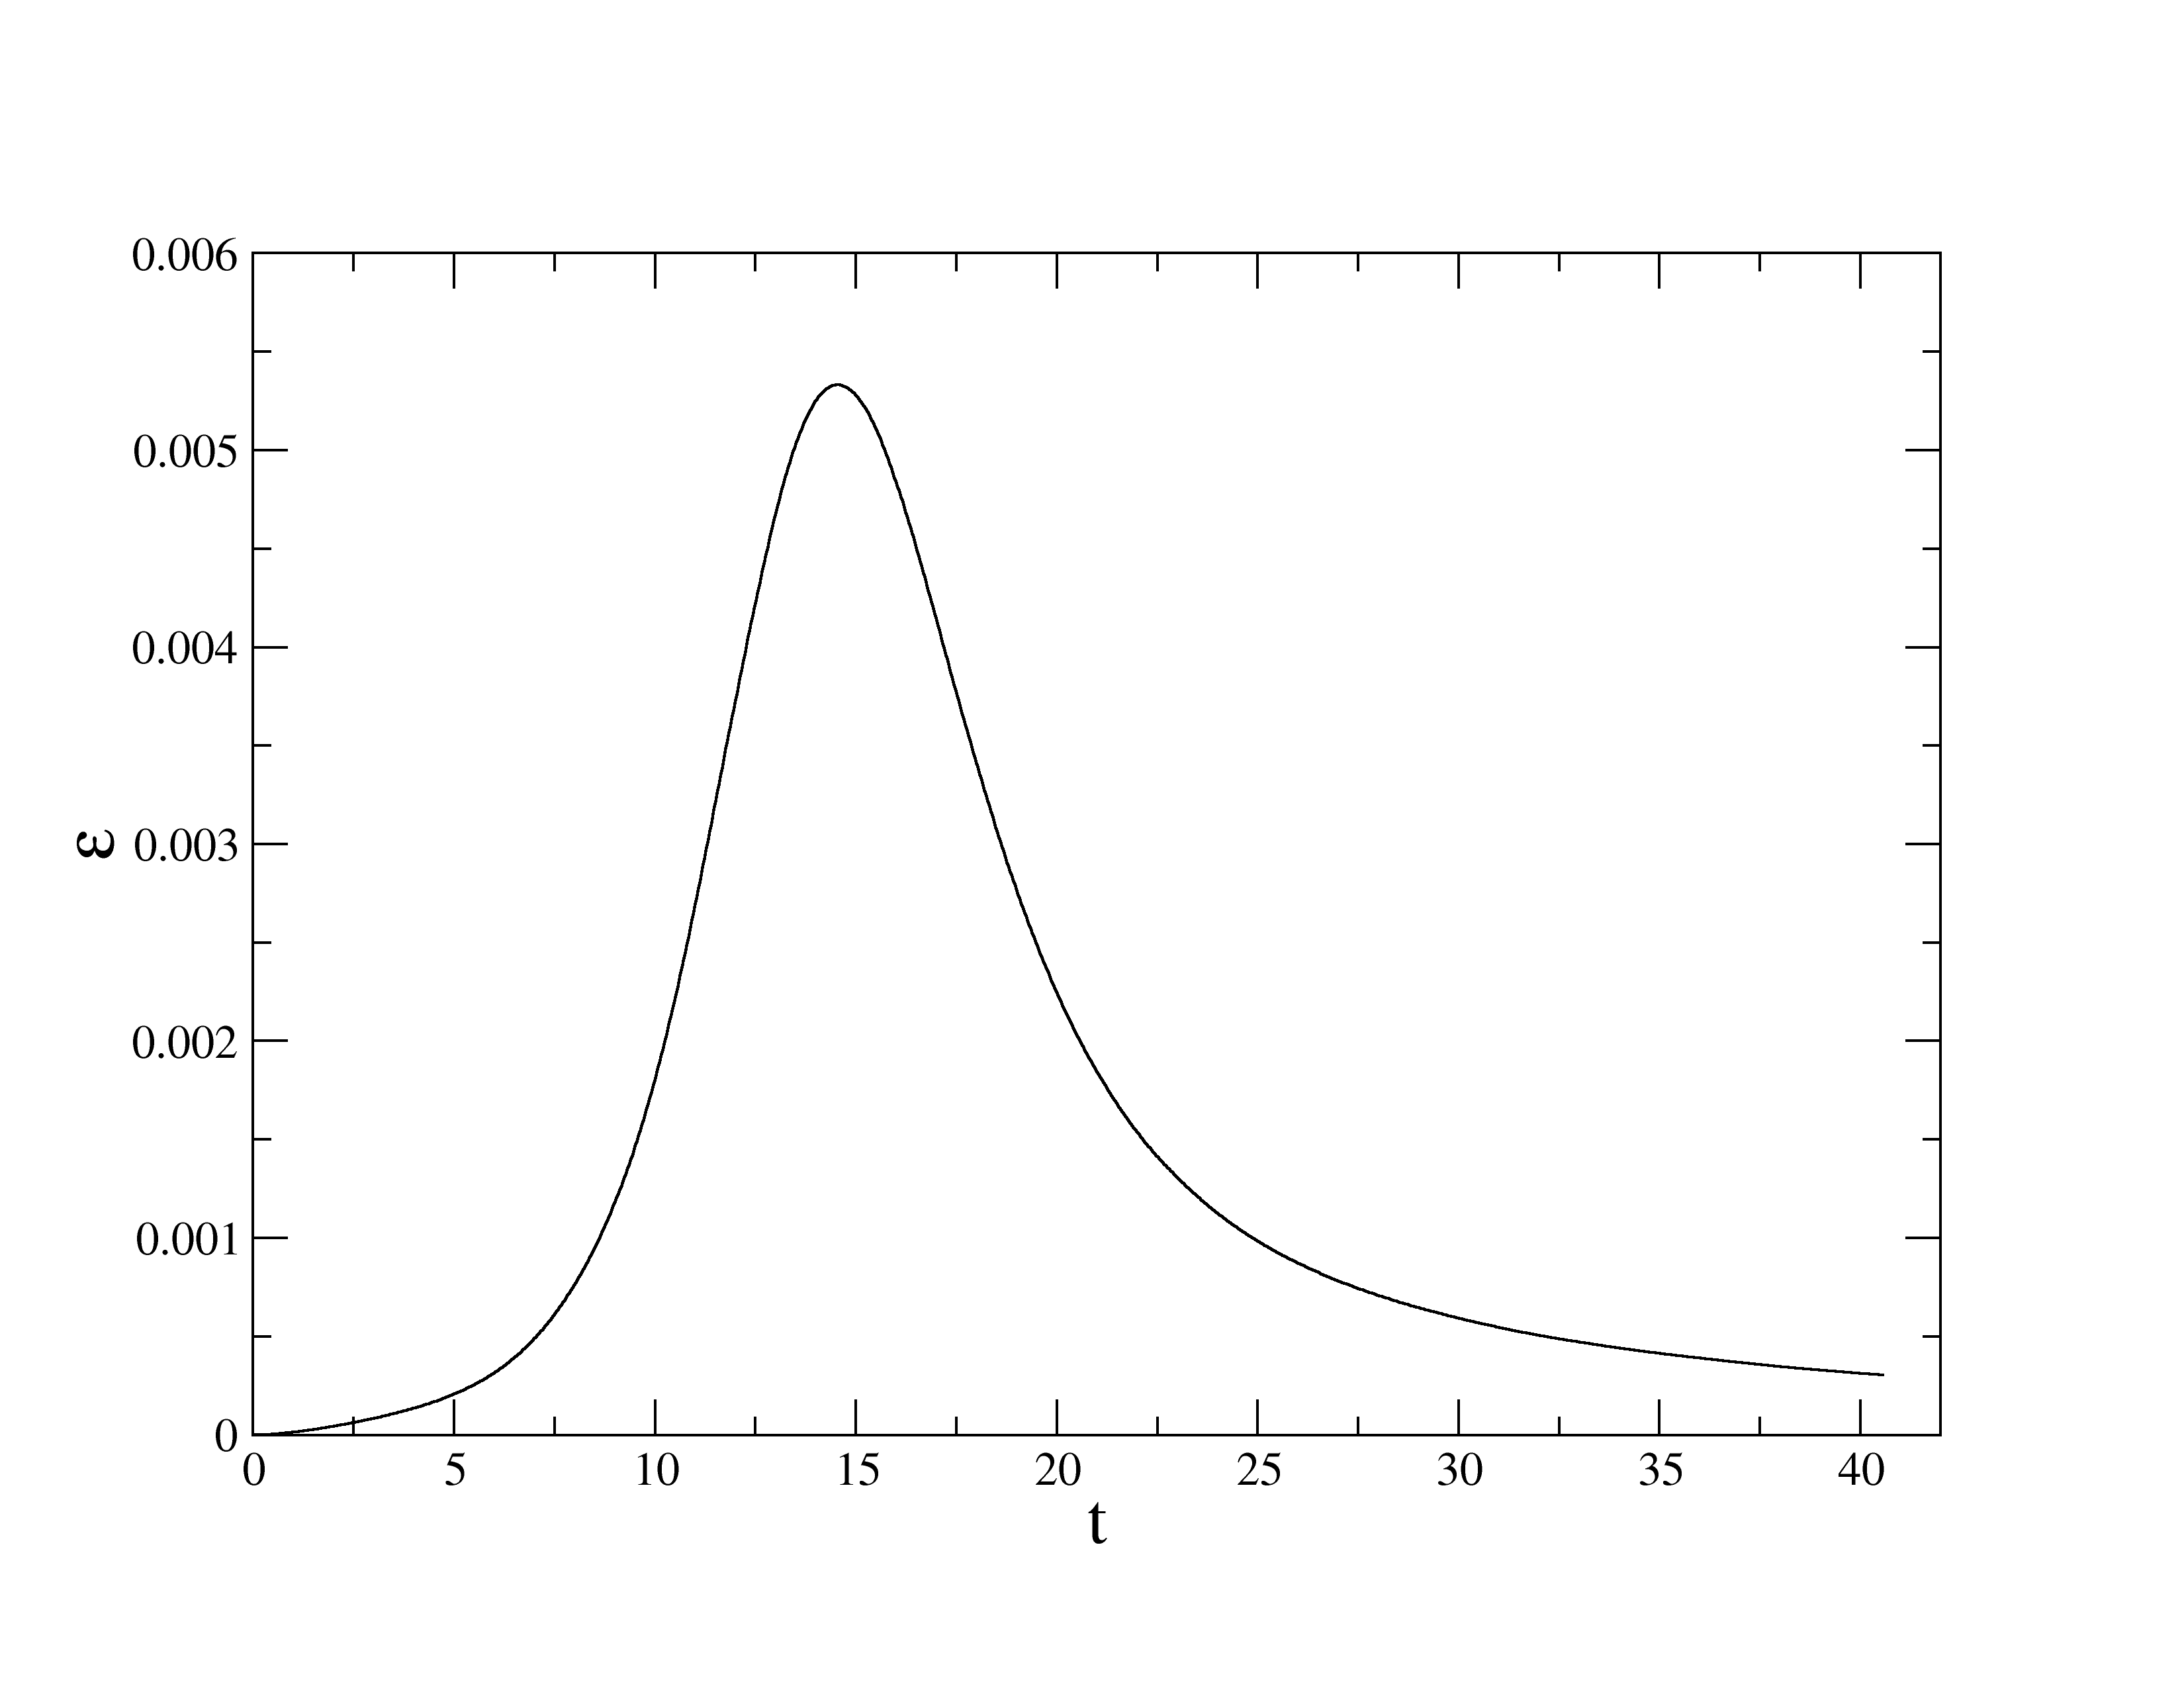
\includegraphics[width=4.5in,clip]{eps.png}}
\caption{Evolution of Favre turbulent kinetic energy dissipation.}
\label{figure4}
\end{figure}

\begin{figure}[h]
\center{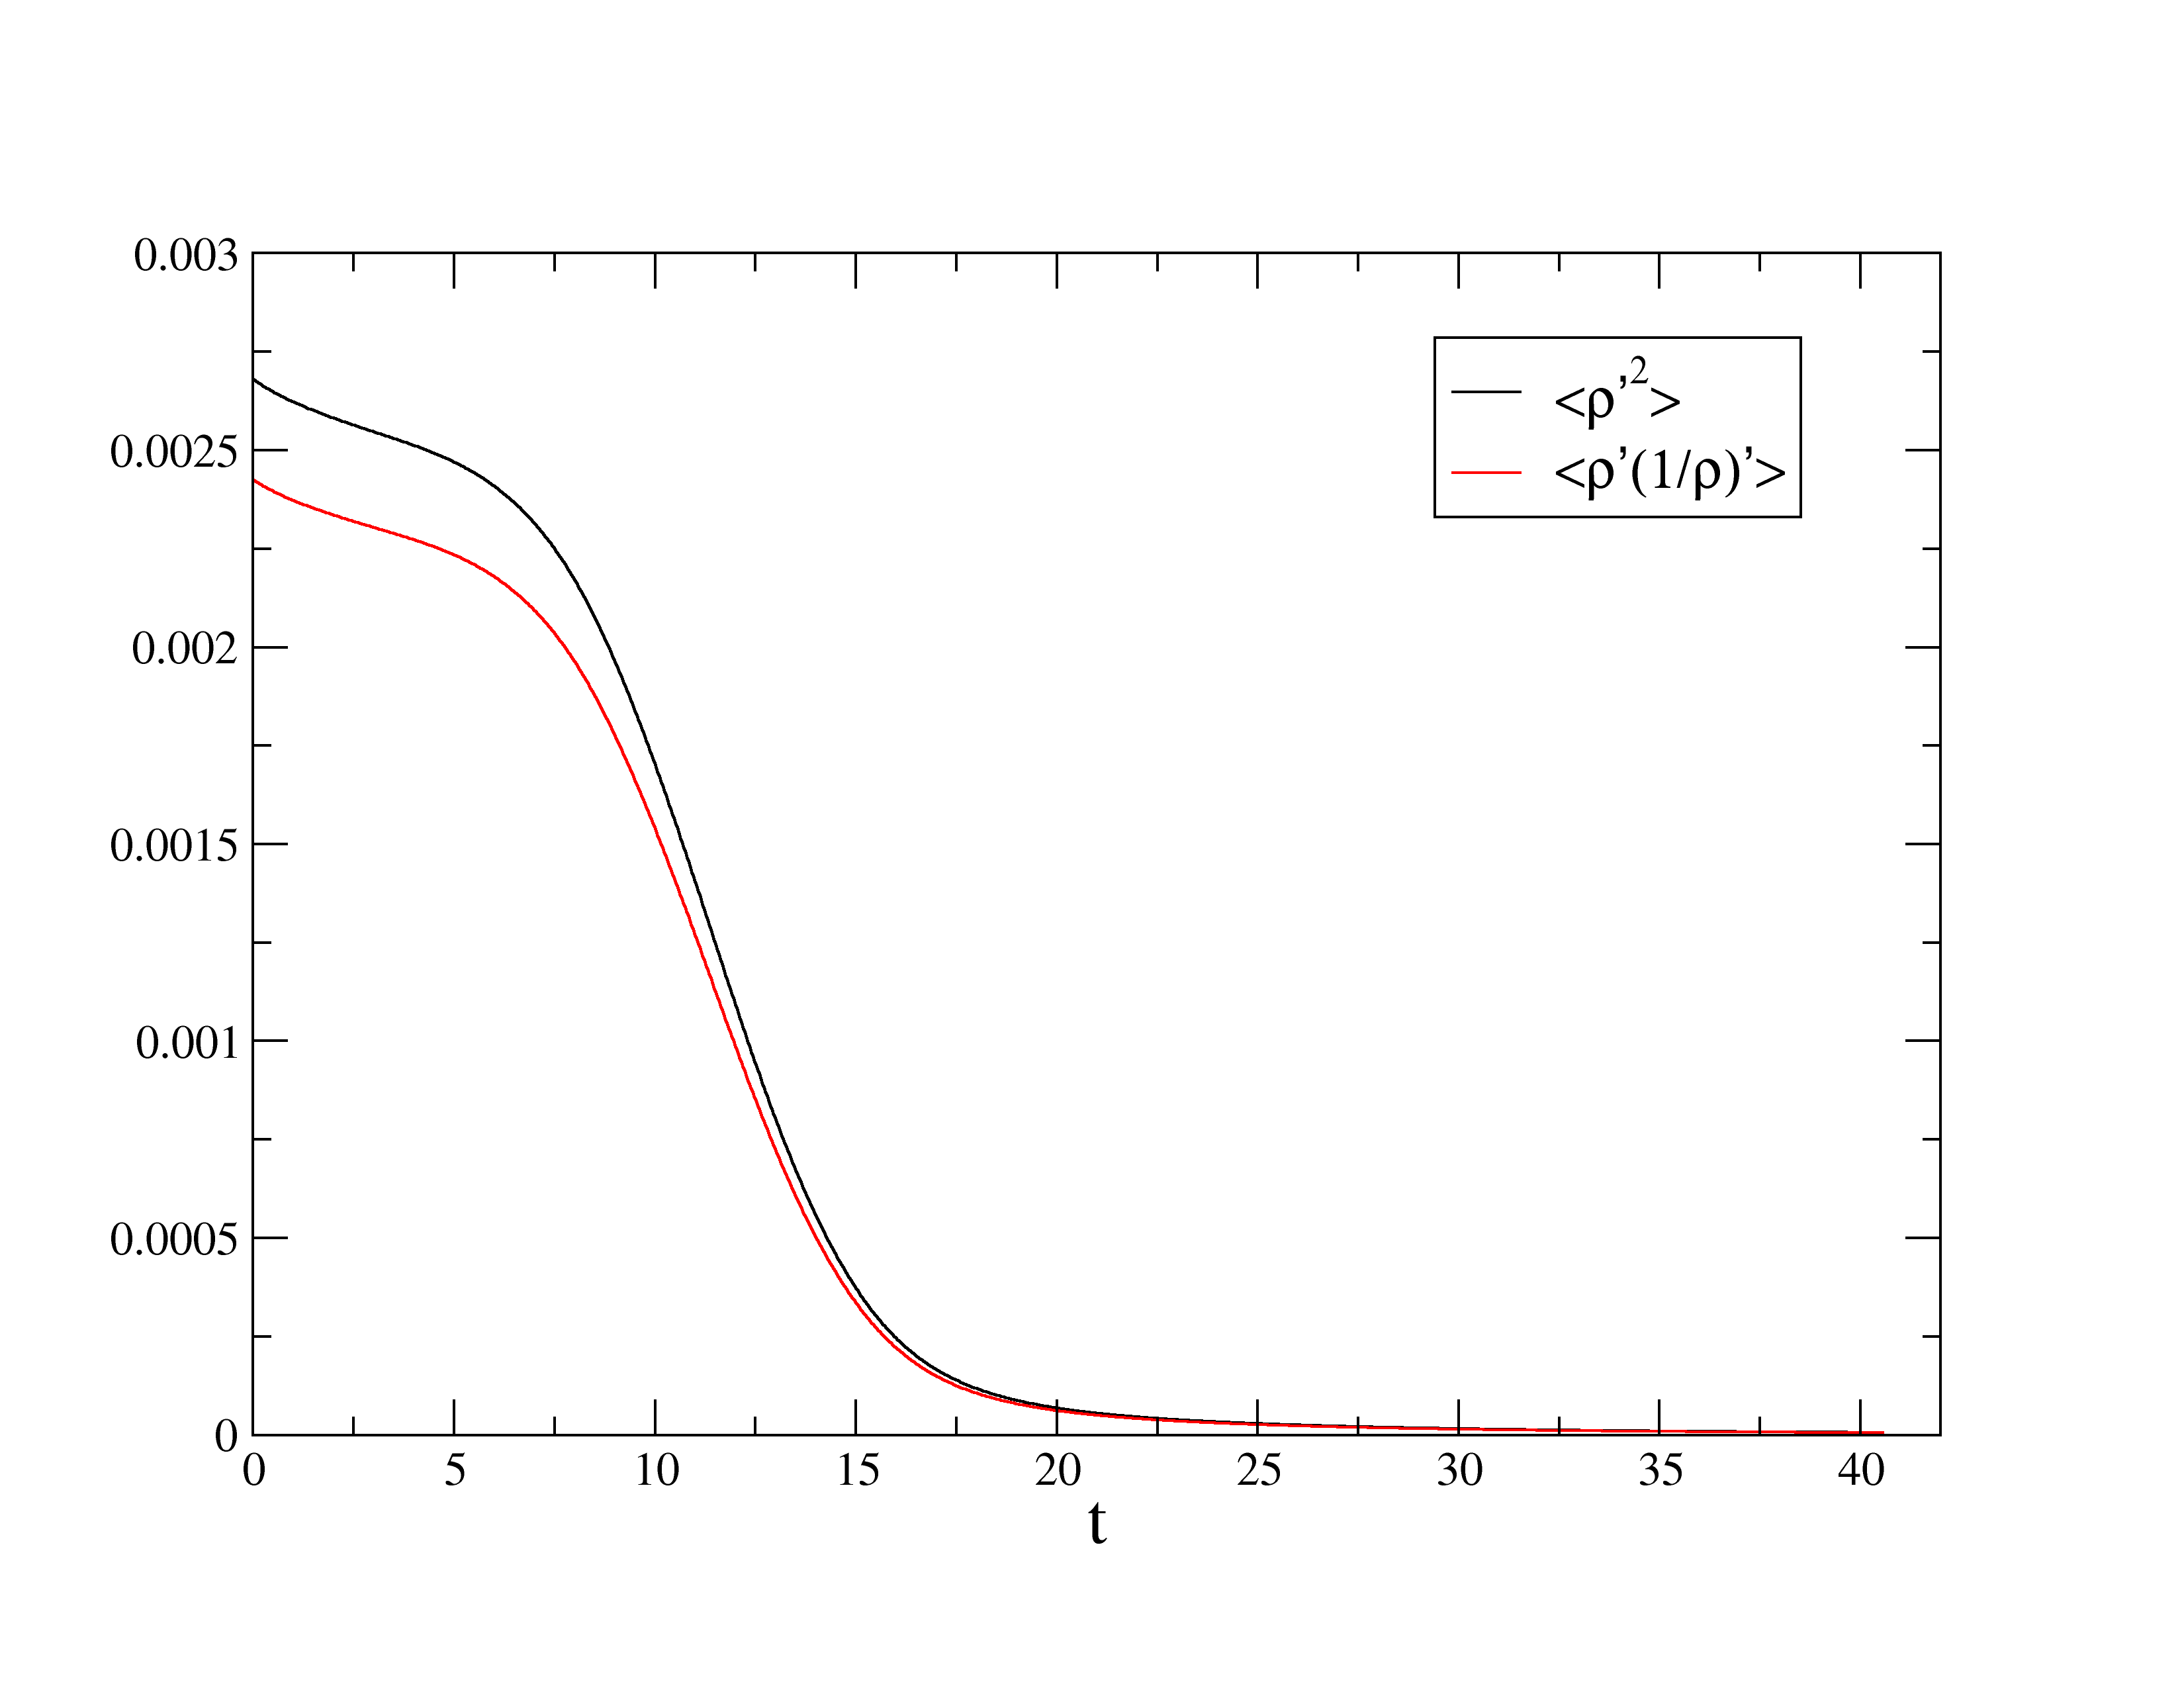
\includegraphics[width=4.5in,clip]{rvar.png}}
\caption{Evolution of density variance and density-specific volume 
correlation.}
\label{figure5}
\end{figure}


\begin{figure}[h]
\center{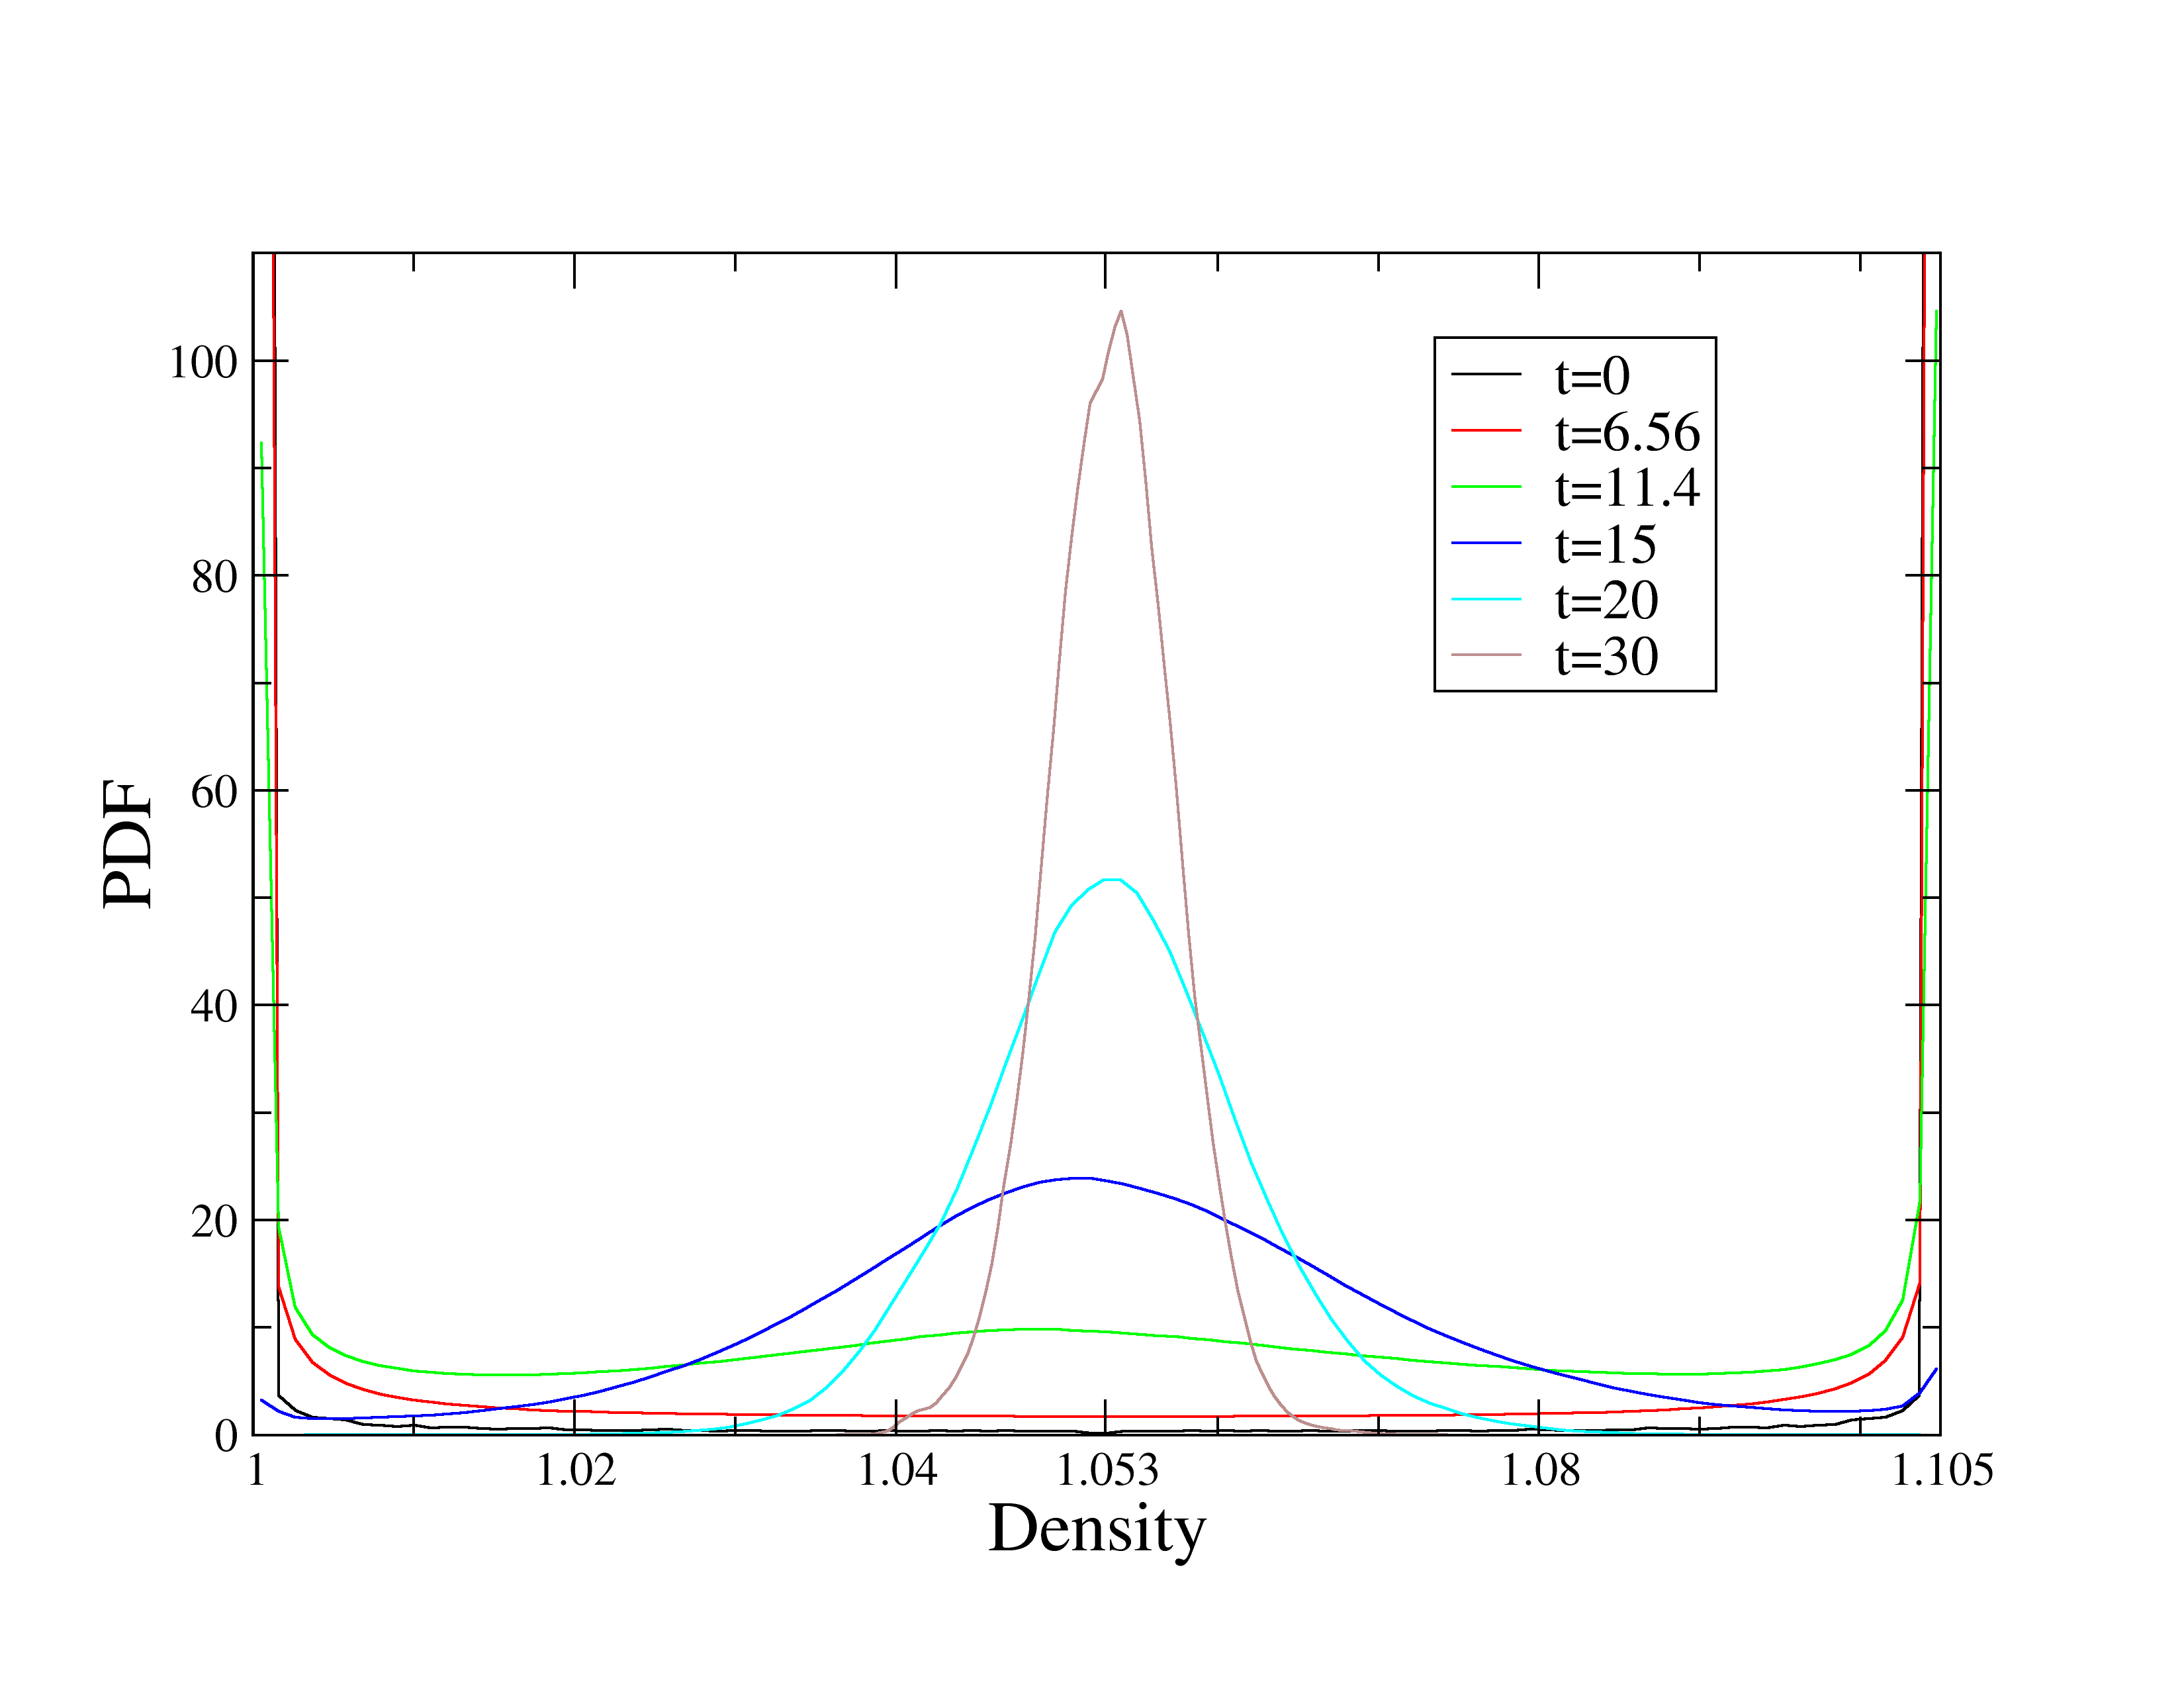
\includegraphics[width=4.5in,clip]{pdf.png}}
\caption{Density PDF at different times.}
\label{figure6}
\end{figure}

\begin{figure}[h]
\center{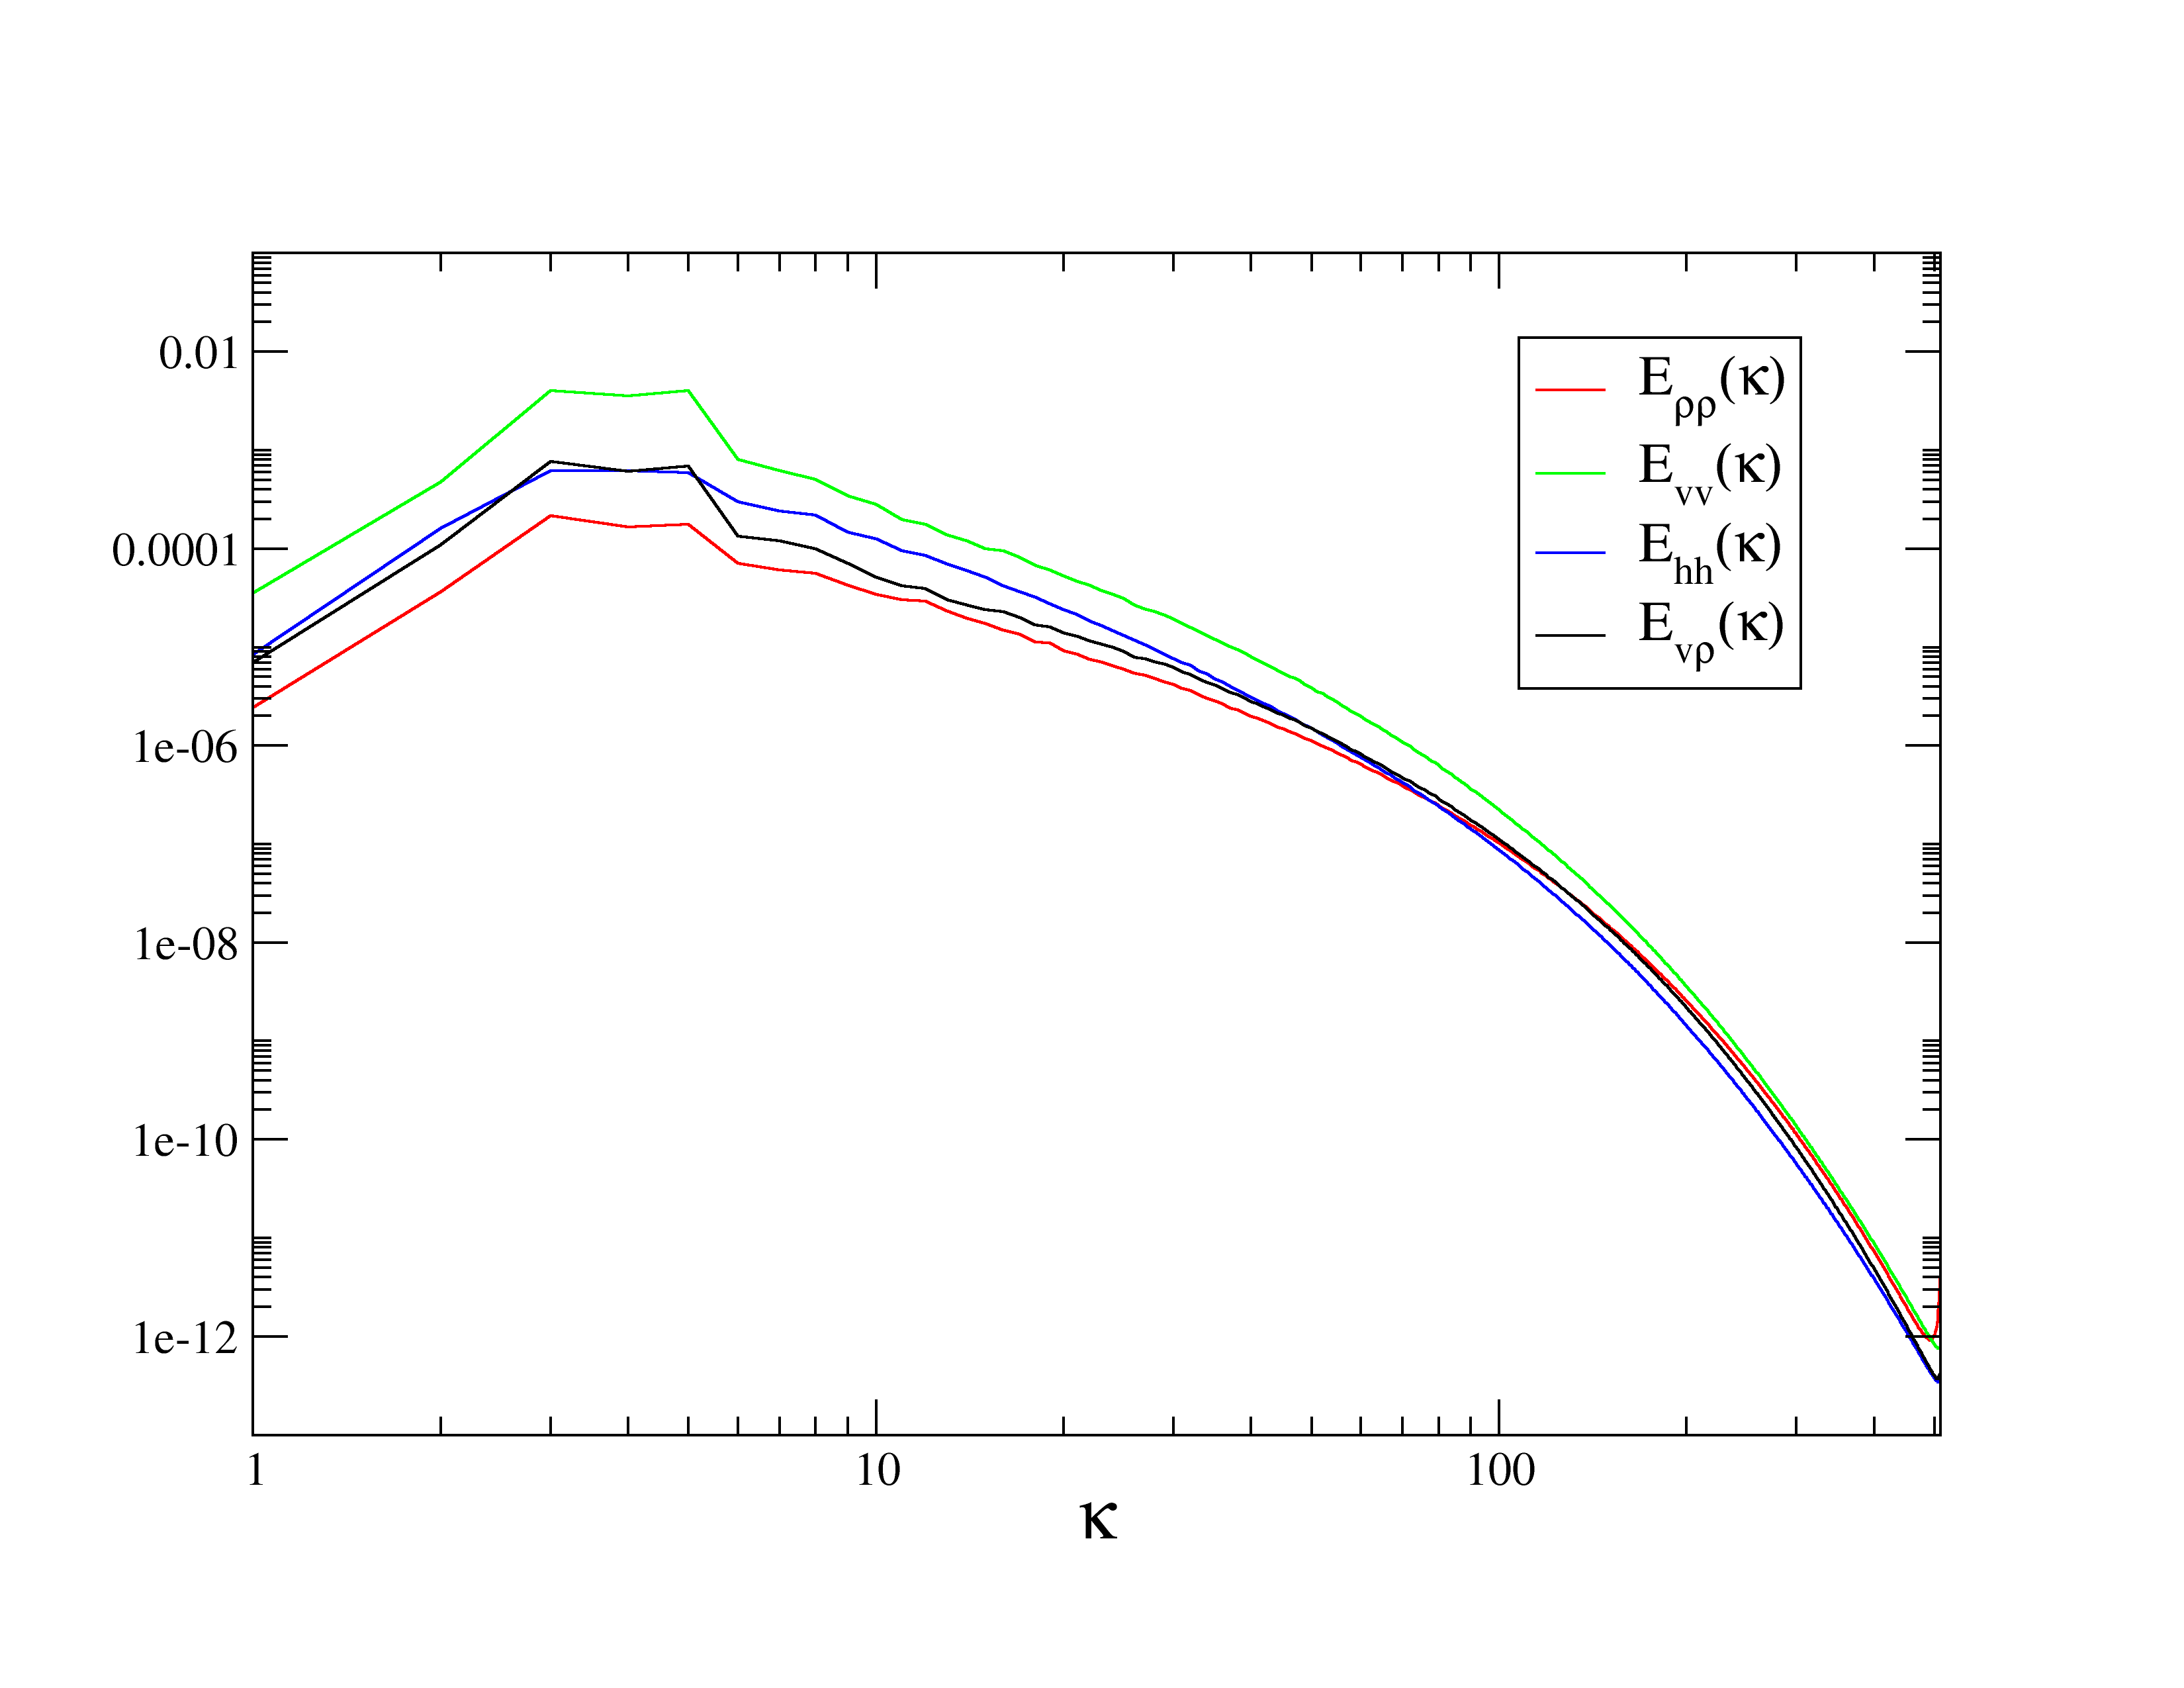
\includegraphics[width=4.5in,clip]{spectra2.png}}\\
\center{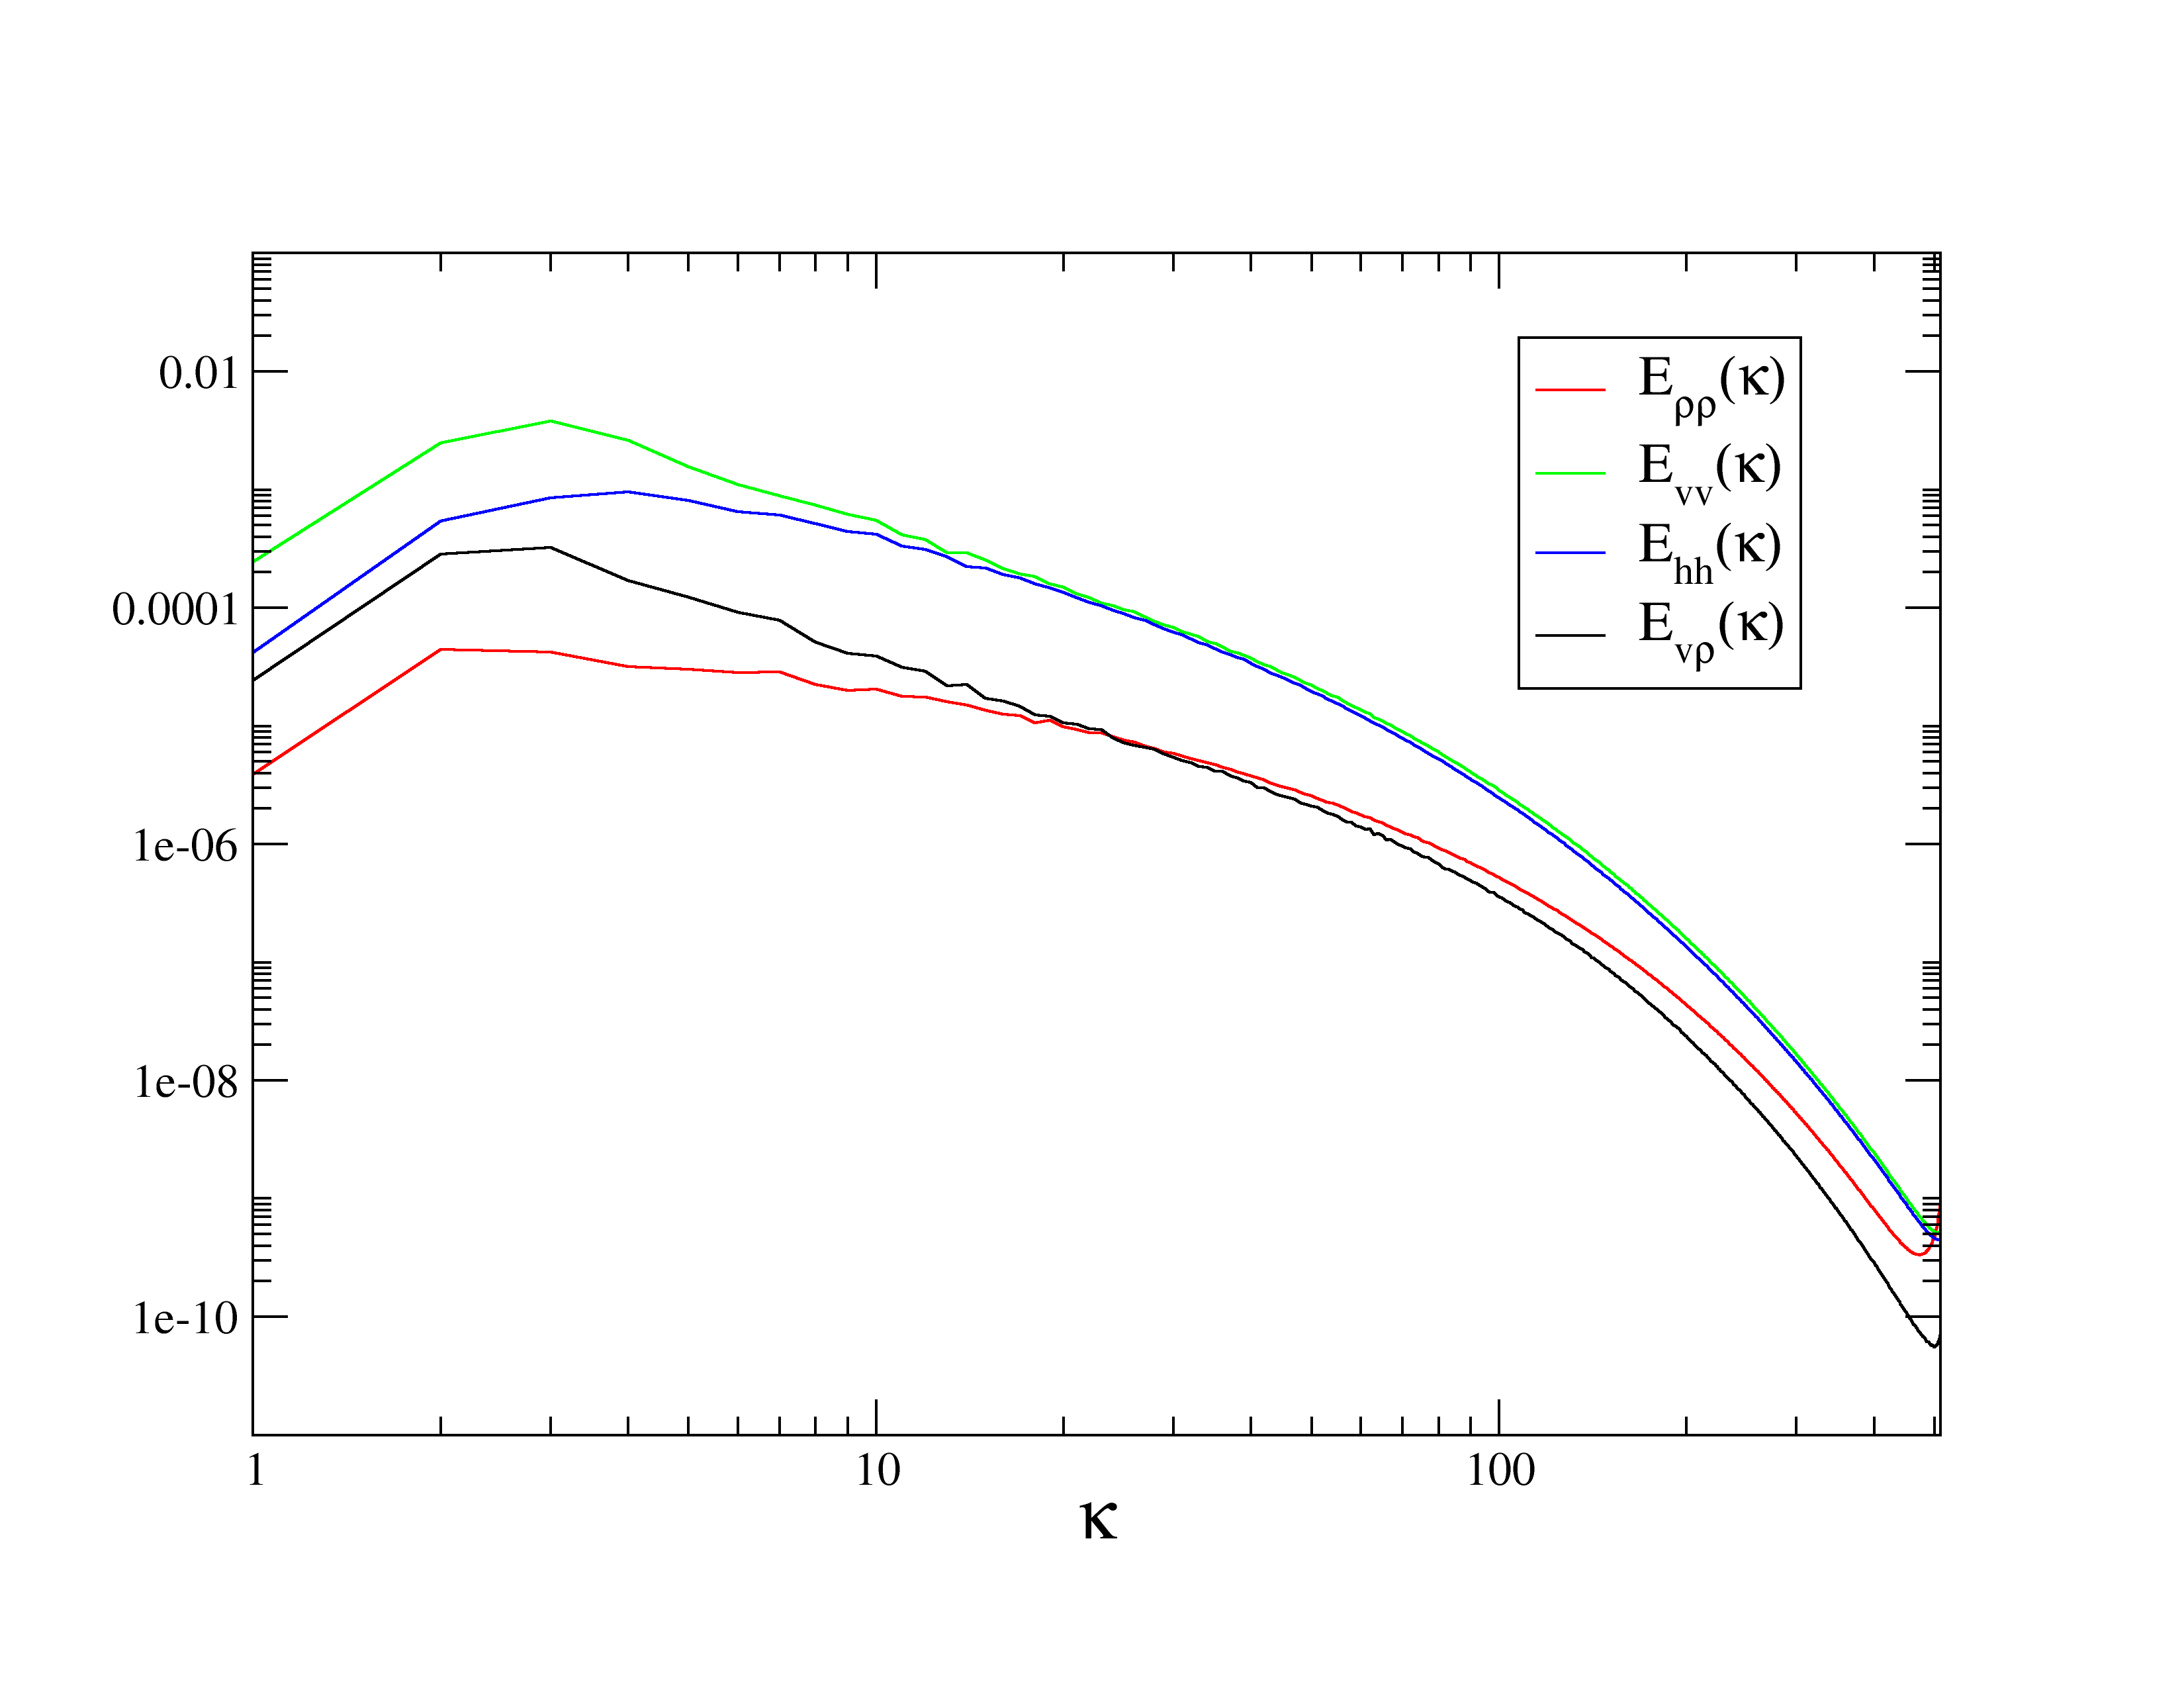
\includegraphics[width=4.5in,clip]{spectra3.png}}
\caption{3-D power spectra of density, $E_{\rho\rho}$, vertical and horizontal 
velocity components, $E_{vv}= E_{11}$ and $E_{hh}= (E_{22}+E_{33})/2$, and 
density vertical velocity co-spectrum, $E_{v\rho}$, at a) t=6.56 (maximum 
$Re_t$) and b) t=11.4 (maximum $\tilde{k}$).
}
\label{figure7}
\end{figure}


\end{document}
